% Requirements 1 and 2(a); numbered equations retain their original order.
\section[Freezer: service efficiency]{Understanding Cooling Efficiency}
\label{sec:understand}

An open freezer succeeds by preserving food, not simply by removing heat. Low electricity use can accompany inadequate storage, while large cooling loads may reflect infiltration through the opening. We therefore evaluate \emph{useful service per unit energy}.

\begin{figure}[!ht]
\centering
\begin{minipage}[c]{0.48\linewidth}
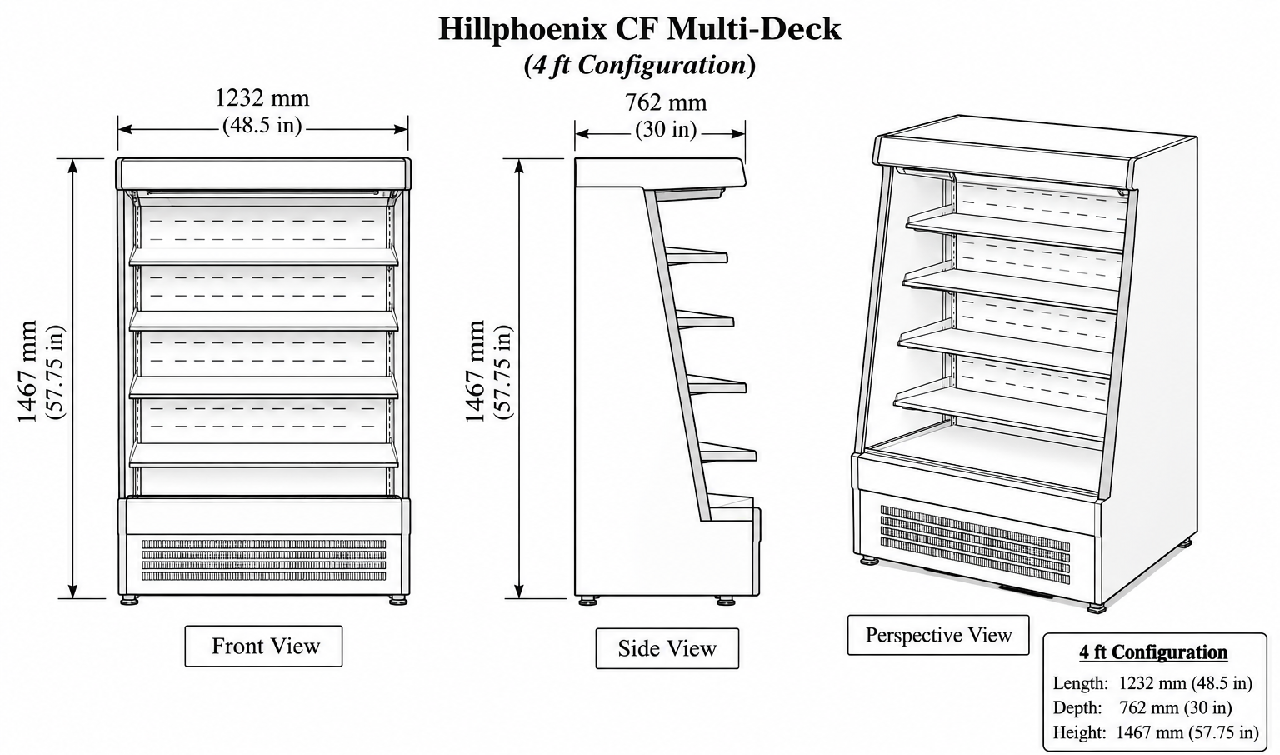
\includegraphics[width=\linewidth]{figures/09_open_display_case.pdf}
\end{minipage}\hfill
\begin{minipage}[c]{0.48\linewidth}
\small
The open front admits warm, moist air; cabinet surfaces conduct and radiate heat. Lights, fans, restocking and defrost add operating loads. Insulation and equipment condition modify these mechanisms; equipment age is not a separate score \cite{ashrae}. Product temperatures must be checked across shelves, since a mean can conceal a warm location \cite{etl}.
\end{minipage}
\caption{Open-case heat pathways and product locations. The supplied medium-temperature display schematic illustrates geometry; freezer limits remain product-specific \cite{hillphoenix}.}
\label{fig:open-case}
\end{figure}

The numerator needs \textbf{quantity, local quality and duration}: compliant product mass integrated over storage time. The denominator includes refrigeration and auxiliaries without overlapping meter readings. Matched loading, ambient conditions and complete operating cycles prevent short operation or stored cold from inflating efficiency:
\begin{equation}
\boxed{\text{Cooling efficiency}
=\frac{\text{useful service accumulated over objects and time}}
{\text{energy input over the same period}}.}
\label{eq:principle}
\end{equation}
\begin{equation}
 \eta_f=\frac{\int\sum_i m_i(t)\mathbf{1}\{T_{p,i}(t)\in\mathcal T_i\}\,dt}
 {\int p_f(t)\,dt},
\label{eq:freezer-service}
\end{equation}
Here $m_i$ is product mass (kg), $\mathcal T_i$ its admissible temperature range, $t$ is hours and $p_f$ is kW; thus $\eta_f$ is compliant kg$\cdot$h/kWh. For people, the response changes to thermal-discomfort relief weighted by occupied time. These recipient-specific numerators cannot be directly compared numerically.

\subsection{A shared physical structure}
For dry-air mass $M_z$ (kg), balanced dry-air streams $\dot m_{jz}$ (kg/s), enthalpy $h$ (J/kg dry air) and humidity ratio $w$ (kg vapor/kg dry air),
\begin{align}
 M_z\dot h_z&=\sum_j\dot m_{jz}(h_j-h_z)+S_{h,z},\\
 M_z\dot w_z&=\sum_j\dot m_{jz}(w_j-w_z)+S_{w,z}.
\label{eq:common-balance}
\end{align}
$S_h$ (W) and $S_w$ (kg/s) contain the appropriate device, occupant, product and surface sources. Freezer refrigeration can remove heat and condensate; public cooling changes airflow and moisture. The bus fixes the background and solves local delivery; the station retains that calculation while resolving background and surface storage \cite{epzone}. Figure~\ref{fig:inheritance} shows this progression. Cruz-Salas et al.\ motivate separating treatment, transport and occupied-space conditions \cite{cruz2026}.

\begin{figure}[!ht]
\centering
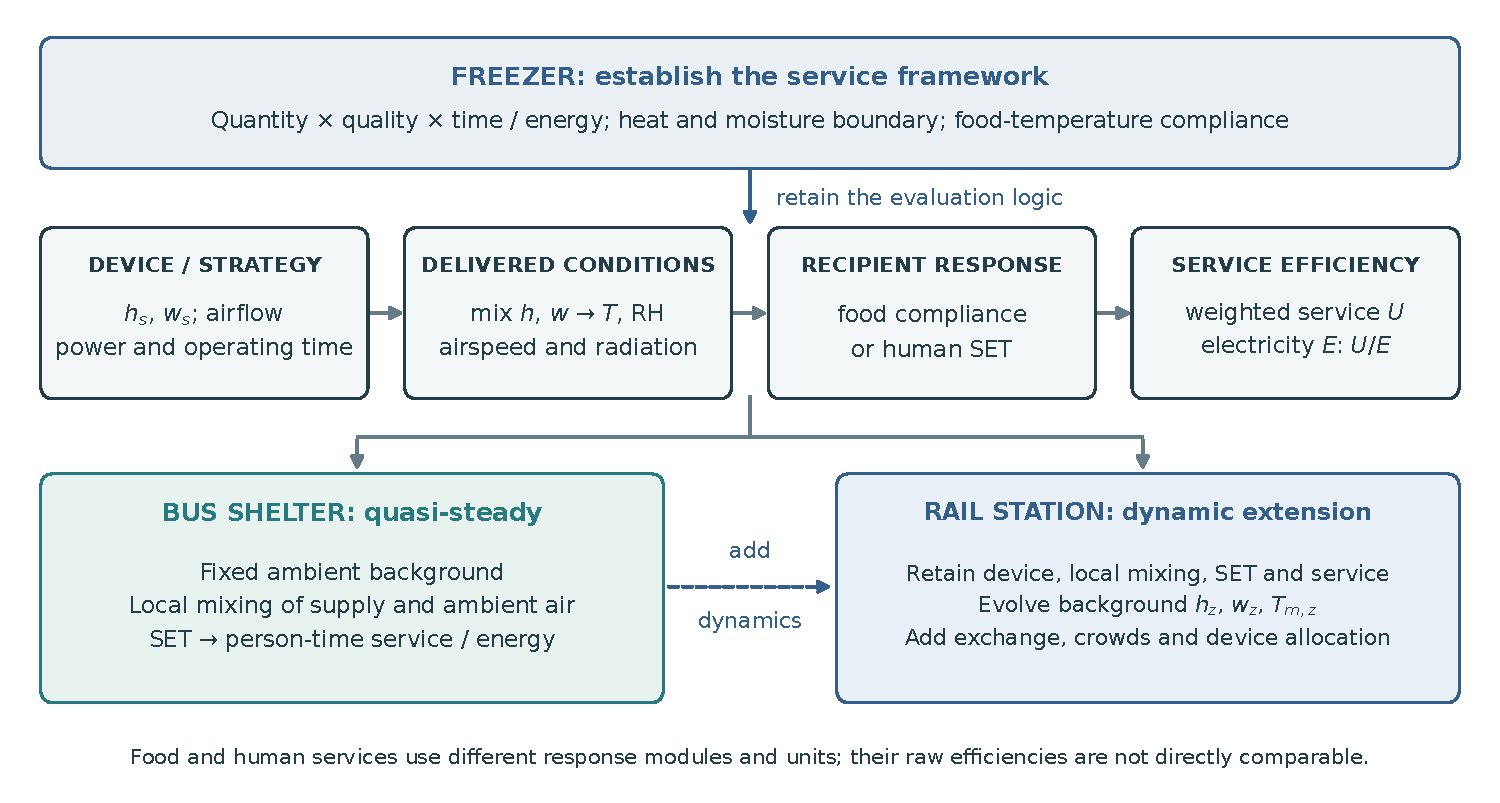
\includegraphics[width=0.94\linewidth]{figures/19_model_inheritance.pdf}
\caption{Shared conservation and service accounting, with recipient-specific response and increasingly resolved background dynamics.}
\label{fig:inheritance}
\end{figure}

\section[Bus shelter]{Bus Stop: Local Delivery and Cooling Efficiency}
\label{sec:bus}

\subsection{Geometry and comparison inputs}
NYC DOT's regular shelter measures $14$ ft by $5$ ft by $8$ ft $11$ in, or $4.2672\times1.5240\times2.7178$ m \cite{nycshelter}. Its gross footprint is $A=6.5032\,\mathrm{m^2}$. Three equal strips have $A_z=2.1677\,\mathrm{m^2}$ and centers $(x_z,W/2)$, $x_z=(z-\tfrac12)L/3$; delivery originates at $x=0$.

\begin{figure}[!ht]
\centering
\begin{minipage}[t]{0.49\linewidth}
\centering
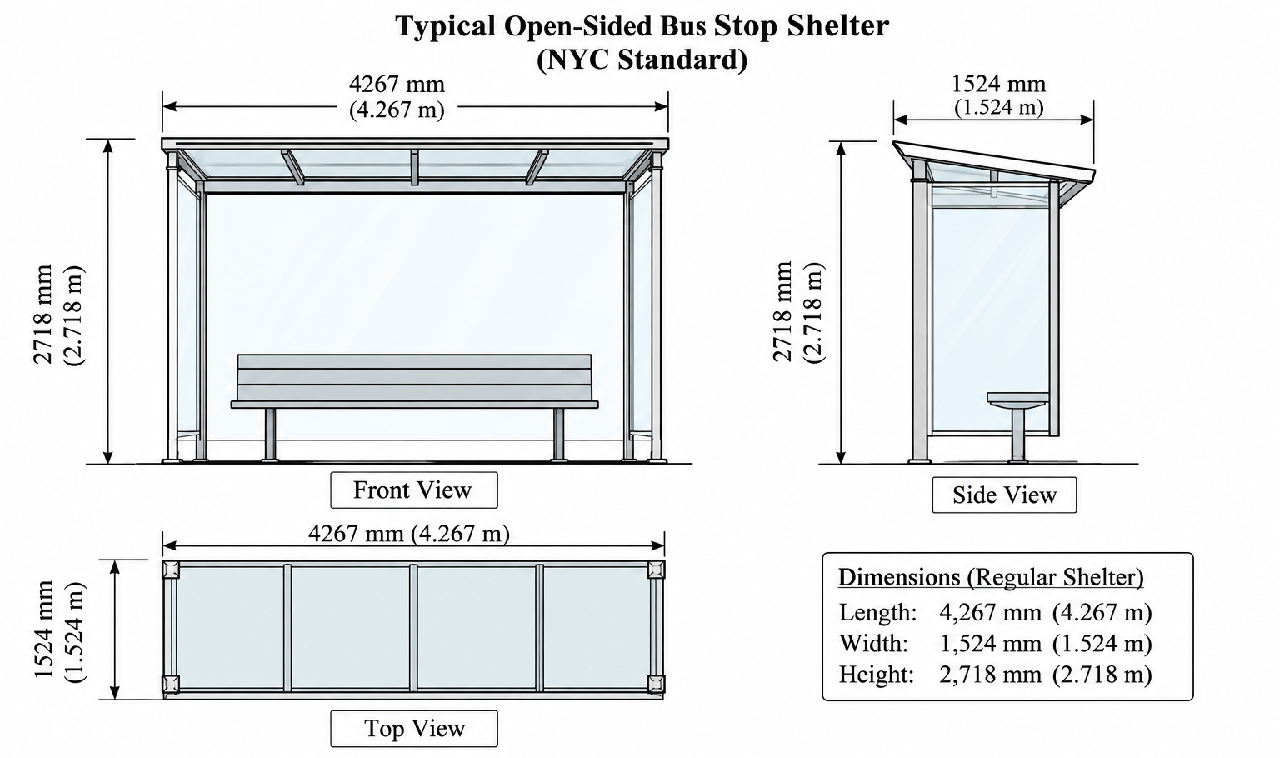
\includegraphics[width=\linewidth]{figures/07_bus_shelter_geometry.pdf}
\caption{Adopted NYC shelter dimensions \cite{nycshelter}.}
\label{fig:shelter-geometry}
\end{minipage}\hfill
\begin{minipage}[t]{0.49\linewidth}
\centering
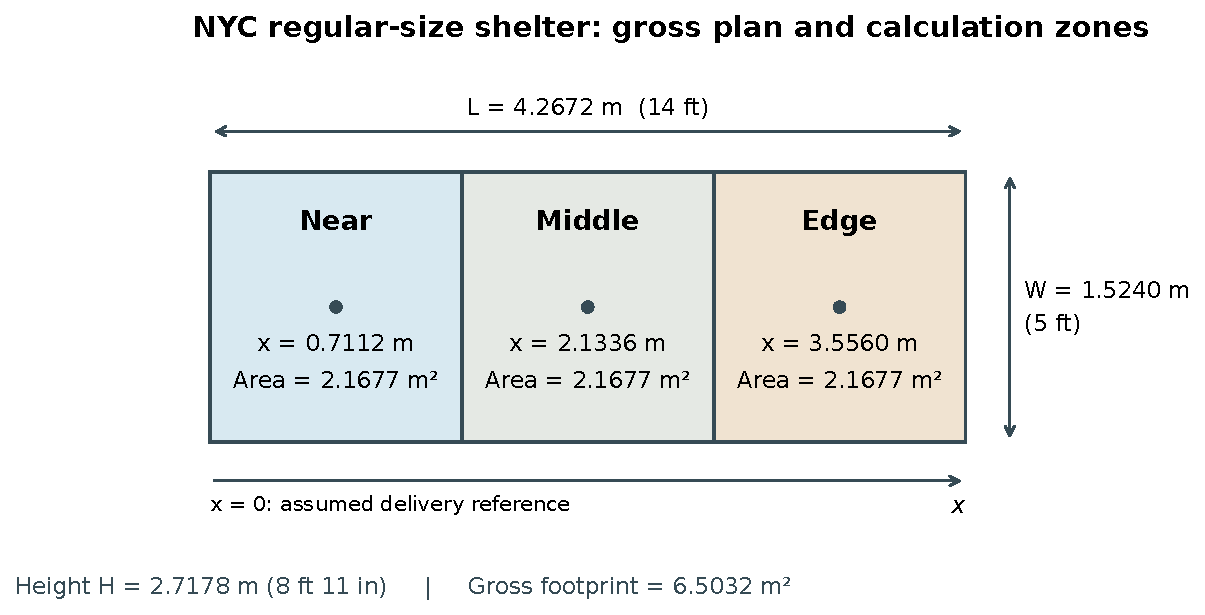
\includegraphics[width=\linewidth]{figures/08_shelter_zoning.pdf}
\caption{Equal near/middle/edge accounting strips.}
\label{fig:shelter-zones}
\end{minipage}
\end{figure}

The problem's $3\,^{\circ}\mathrm C$ fan effect describes perceived cooling; B/C's $5/8\,^{\circ}\mathrm C$ describe air cooling \cite{problem}. We interpret the listed kW/hr numbers as powers $p_{A/B/C}=0.25/1.2/2.5$ kW. Tables~\ref{tab:bus-assumptions}--\ref{tab:bus-fields} specify the comparison: $34\,^{\circ}\mathrm C$, RH $30/70\%$, $T_r=36\,^{\circ}\mathrm C$ and 12 mean occupants. Geometry enters once through $n_z=\rho_zA_z$ when density replaces headcount.

\subsection{From device outlet to occupied air}
A changes prescribed local speed while retaining background temperature and moisture in the zero-local-heat base case \cite{fanguide}. For B/C, wet-bulb temperature bounds evaporation \cite{evapequip}:
\begin{equation}
 T_{o,s}=T_b-\min\{\Delta T_s^{\max},\;\varepsilon_s(T_b-T_{wb,b})\},
 \qquad s\in\{B,C\},
\label{eq:outlet}
\end{equation}
$b$ denotes the inlet background; $\varepsilon_s$ is evaporative effectiveness and $\Delta T_{B/C}^{\max}=5/8\,^{\circ}\mathrm C$ are the adopted outlet caps. With $\phi$ as RH fraction and pressures in Pa, SI psychrometrics give \cite{psychrolib}
\begin{align}
 w&=0.621945\frac{p_v}{p-p_v},\qquad p_v=\phi p_{sat}(T),\\
 h(T,w)&=1006T+w(2501000+1860T),
\label{eq:enthalpy}
\end{align}
Temperatures are in $^{\circ}$C. The near-isenthalpic evaporative stage, $h_{o,s}\simeq h_b$, yields
\begin{equation}
 w_{o,s}=\frac{h_b-1006T_{o,s}}{2501000+1860T_{o,s}}.
\end{equation}
This stage precedes electrical heating and neglects make-up-water enthalpy \cite{evap}. A device supply mixes with entrained background in a negligible-storage local region. For $x\in\{h,w\}$,
\begin{equation}
 0=\dot m_{s,z}(x_s^{\rm sup}-x_{\ell,s,z})+
 \dot m_{e,z}(x_b-x_{\ell,s,z}),\qquad
 \beta_{s,z}=\frac{\dot m_{s,z}}{\dot m_{s,z}+\dot m_{e,z}}.
\label{eq:delivery-balance}
\end{equation}
$\beta$ is a dry-air flow fraction, not a fraction of passengers or total flow assigned to a strip. A fraction $\chi$ of unit electric power $P_s=1000p_s$ W heats unit supply flow $\dot m_s$ before reaching people:
\begin{equation}
 h_s^{\rm sup}=h_{o,s}+\chi P_s/\dot m_s,\qquad
 w_s^{\rm sup}=w_{o,s},\qquad 0\leq\chi\leq1.
\label{eq:supply-heat}
\end{equation}
For A, the unheated outlet equals the inlet. Mixing conserves $h,w$, after which temperature and RH are recovered:
\begin{align}
 w_{\ell,s,z}&=(1-\beta_{s,z})w_b+\beta_{s,z}w_s^{\rm sup},\\
 h_{\ell,s,z}&=(1-\beta_{s,z})h_b+\beta_{s,z}h_s^{\rm sup},\\
 T_{\ell,s,z}&=\frac{h_{\ell,s,z}-2501000w_{\ell,s,z}}{1006+1860w_{\ell,s,z}}.
\label{eq:mixing}
\end{align}
RH is not averaged directly. The bus uses $b=a$ and $\chi=0$. Its B/C fractions imply entrainment-to-supply ratios $(1-\beta)/\beta=0.25/1.22/9.00$ and $0.11/0.43/1.50$. Parallel strip branches share one device's total supply.

\subsection{A common response and efficiency measure}
Standard effective temperature (SET) combines air temperature, radiation, airspeed and humidity for the reference passenger \cite{thermalcomfort,pythermal}:
\begin{equation}
 \Theta_{s,z}=F_{\mathrm{SET}}(T_{\ell,s,z},T_{r,z},v_{s,z},\phi_{\ell,s,z};\mathrm{met},\mathrm{clo}).
\label{eq:set}
\end{equation}
For the assumed hot-discomfort reference $\Theta_c=26\,^{\circ}\mathrm C$, define
\begin{equation}
 D(\Theta)=[\Theta-\Theta_c]_+,\qquad [x]_+=\max(x,0).
\end{equation}
Against the same shelter without active cooling, the signed improvement is
\begin{equation}
 b_{s,z,k}=D(\Theta_{0,z,k})-D(\Theta_{s,z,k}).
\end{equation}
Adverse effects remain negative. With $n_{z,k}$ people and time steps $\Delta t_k$ in hours,
\begin{align}
 U_s&=\sum_k\sum_z n_{z,k}b_{s,z,k}\Delta t_k, &
 E_s&=\sum_k p_{s,k}\Delta t_k,\\
 \eta_s&=U_s/E_s,\qquad E_s>0.
\label{eq:bus-efficiency}
\end{align}
Here $E$ is kWh and $\eta$ is person$\cdot{}^{\circ}\mathrm C\cdot$h/kWh, not COP. Empty zones earn no service; the zero-energy baseline has no ratio. The residual provides an accounting check:
\begin{equation}
 R_s=\sum_k\sum_z n_{z,k}D(\Theta_{s,z,k})\Delta t_k,
 \qquad \overline R_s=\frac{R_s}{\sum_k\sum_z n_{z,k}\Delta t_k}.
\label{eq:remaining}
\end{equation}
Thus $U_s+R_s=R_0$. We rank efficiency by $\eta$; overall adequacy enters Section~\ref{sec:effectiveness}. Under common operating time, the power ratios give delivery-independent break-even conditions:
\begin{equation}
\begin{aligned}
 \eta_B>\eta_A&\iff U_B>4.8U_A,\\
 \eta_C>\eta_A&\iff U_C>10U_A,\\
 \eta_C>\eta_B&\iff U_C>\frac{25}{12}U_B.
\end{aligned}
\label{eq:break-even}
\end{equation}

\subsection{Results: humidity and spatial delivery}
\begin{figure}[!ht]
\centering
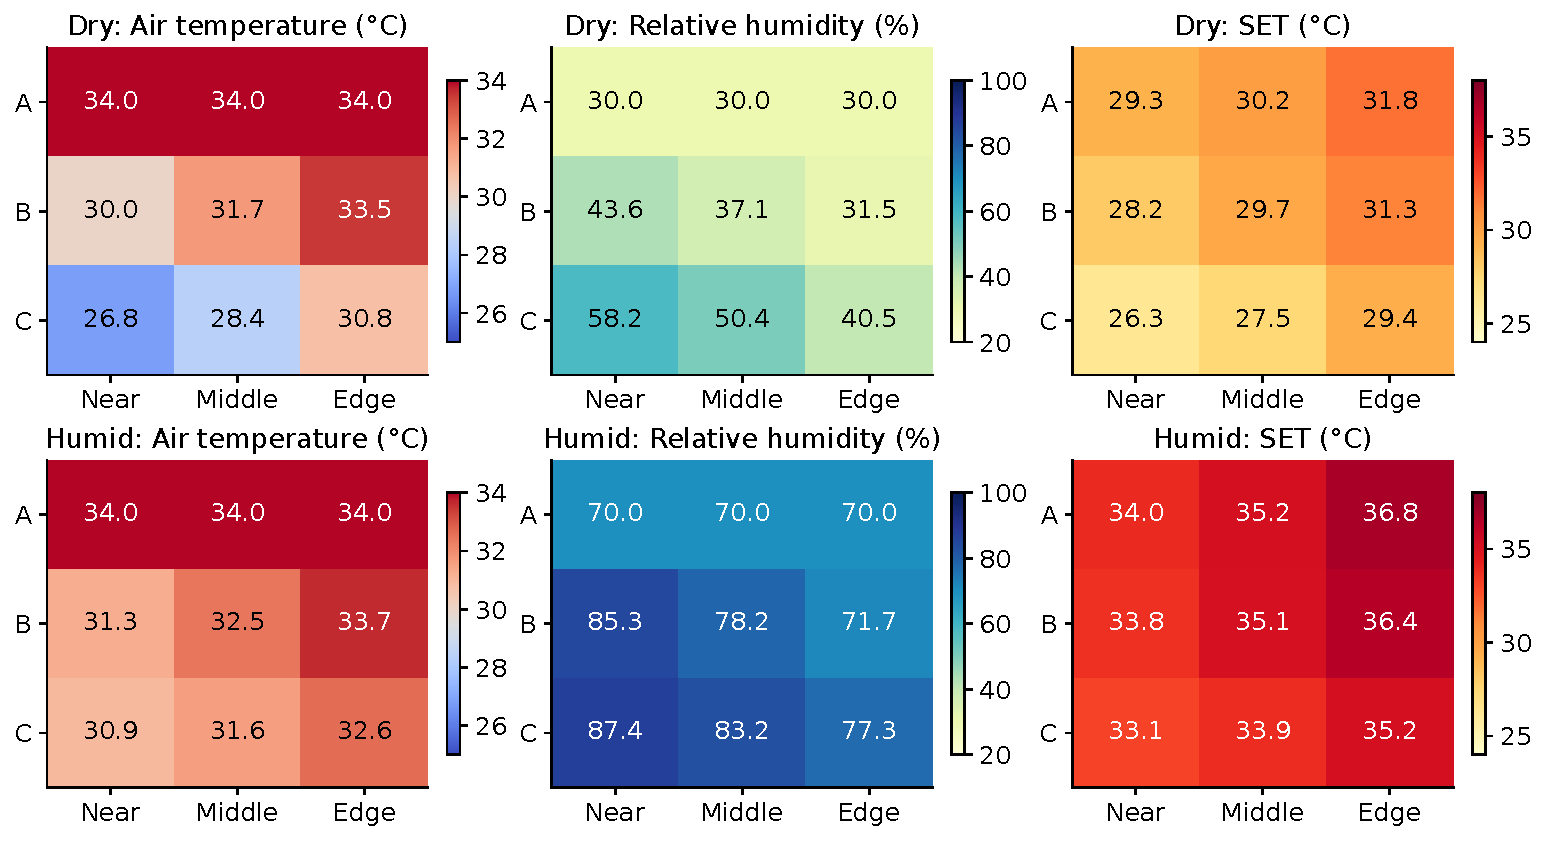
\includegraphics[width=0.88\linewidth]{figures/01_local_conditions.pdf}
\caption{Local conditions under the bus inputs: A changes SET through airflow; B/C also change temperature and moisture.}
\label{fig:bus-local}
\end{figure}
For C, dry-case SET rises from $26.3\,^{\circ}\mathrm C$ near the outlet to $29.4\,^{\circ}\mathrm C$ at the edge; at RH $70\%$, it rises from $33.1$ to $35.2\,^{\circ}\mathrm C$. These gradients explain why a single air-temperature drop misses delivered service.

\begin{figure}[!ht]
\centering
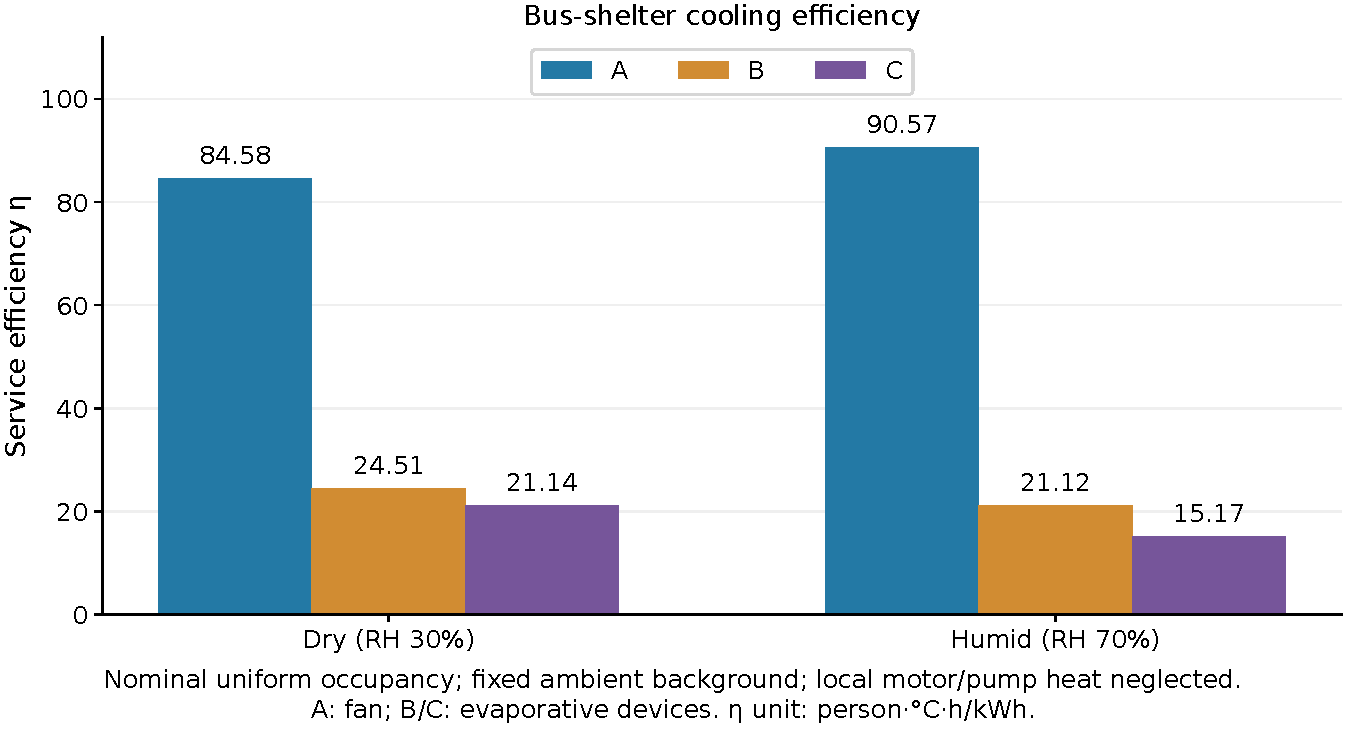
\includegraphics[width=0.76\linewidth]{figures/24_bus_efficiency.pdf}
\caption{Uniform-occupancy efficiency: A leads both nominal humidity cases.}
\label{fig:bus-efficiency}
\end{figure}
Dry-case efficiencies are $84.6/24.5/21.1$ for A/B/C; humid-case values are $90.6/21.1/15.2$ (Figure~\ref{fig:bus-efficiency}). B/C outlet drops fall from $5/8\,^{\circ}\mathrm C$ to about $3.4/3.4\,^{\circ}\mathrm C$, as their common wet-bulb limit replaces the caps.

\begin{figure}[!ht]
\centering
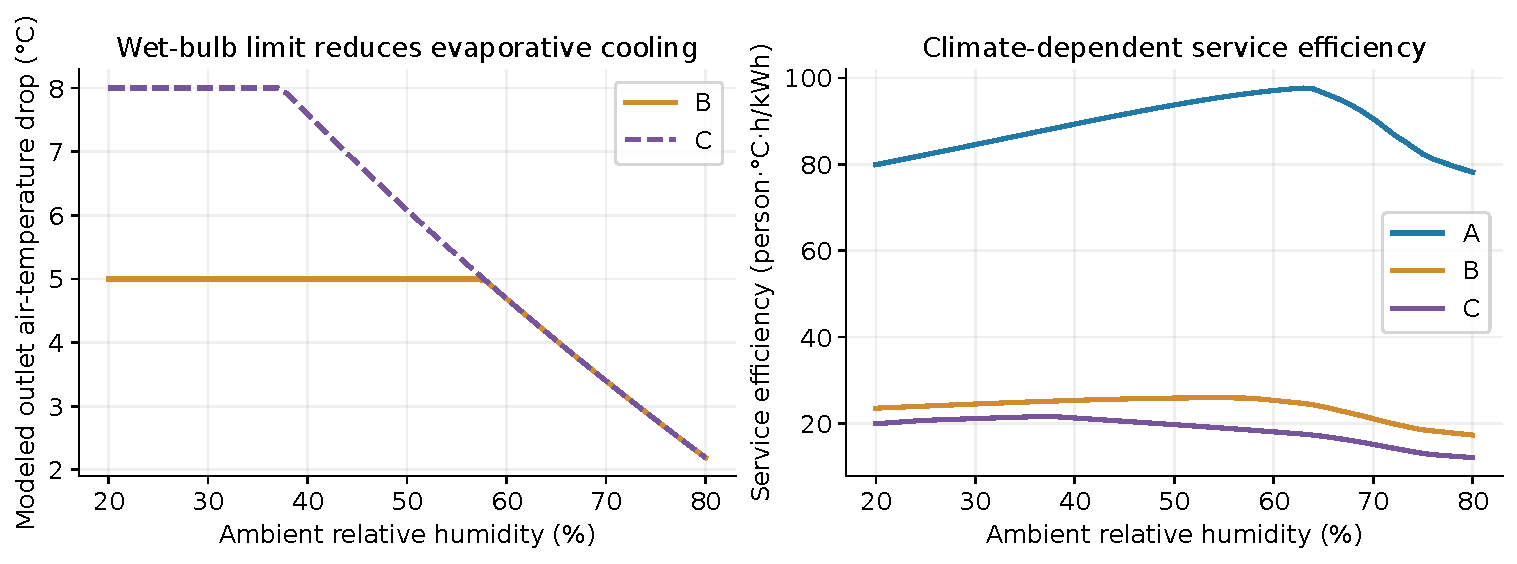
\includegraphics[width=0.88\linewidth]{figures/03_humidity_sweep.pdf}
\caption{Humidity changes evaporative potential and SET-based efficiency at fixed delivery and demand.}
\label{fig:bus-humidity}
\end{figure}
Moving the same 12 people toward the edge lowers dry-case A efficiency from $118.3$ to $48.3$ and reverses B/C ordering: $24.5>21.1$ under uniform occupancy becomes $15.5<16.6$ under edge-heavy occupancy. A leads all six nominal climate--occupancy cases.

\subsection{Delivery failure and robustness}
Aiming or obstruction can weaken delivered airflow without reducing power. Holding $p_A=0.25$ kW, test
\begin{equation}
 v_{A,z}(q)=v_0+q(v_{A,z}^{\mathrm{nom}}-v_0),\qquad 0\leq q\leq1,
\end{equation}
$q$ is a delivery factor, not a motor-speed setting. On the sampled grid, A first wins at $q=0.18$ for RH $30\%$ and $0.16$ for RH $70\%$; the threshold lies within the preceding $0.02$ interval. B wins below it.

\begin{figure}[!ht]
\centering
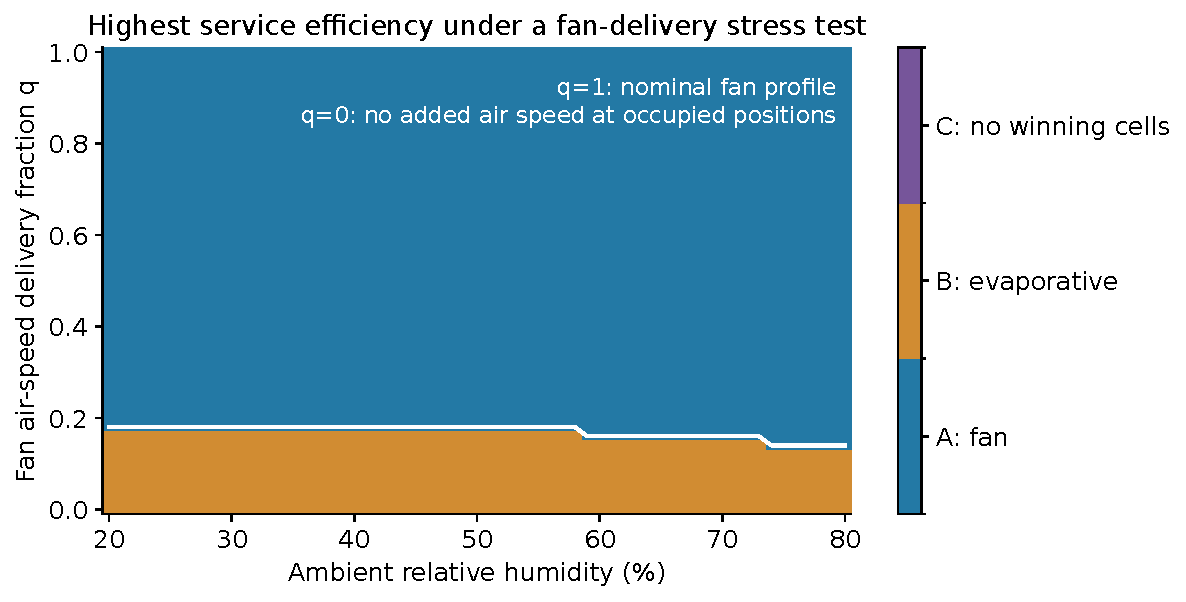
\includegraphics[width=0.79\linewidth]{figures/05_delivery_decision.pdf}
\caption{Efficiency winner for RH $20$--$80\%$ and delivered-speed factor $q$; C wins no cell of this grid.}
\label{fig:bus-decision}
\end{figure}
One-factor endpoint tests give maximum B/A and C/A efficiency ratios $0.432$ and $0.372$. Including full local electric heating ($\chi=1$) changes dry-case efficiencies to $81.0/20.8/18.0$ and humid values to $86.8/17.4/12.1$; A remains first under those inputs. Psychrometric round trips, mass/enthalpy closure, $U+R=R_0$, zero-occupancy and signed-adverse checks pass. The delivery-loss reversal identifies a stronger sensitivity than these individual endpoint perturbations.
\subsection{Extreme dry heat: testing the efficiency ranking}
We test $T_a=T_r=40\,^{\circ}\mathrm C$ at RH 15\% and 20\%, retaining the device powers, delivery profiles, 5/8$\,^{\circ}\mathrm C$ outlet caps, and uniform occupancy. Figure~\ref{fig:extreme-heat} shows $\eta_A>\eta_B>\eta_C$ in both cases. At RH 15\%, the mean SET reductions are 1.43, 1.95, and 3.42$\,^{\circ}\mathrm C$, whereas the efficiencies are 68.43, 19.48, and 16.41 person$\cdot{}^{\circ}\mathrm C\cdot$h/kWh. C produces greater relief per passenger, but consumes ten times A's electricity. SET relief explains the service numerator; $\eta$ remains the comparison criterion.

The heat balance explains why dry-bulb cooling alone cannot establish the ranking. When air is warmer than the exposed skin or clothing surface, faster flow increases convective heat gain; it also promotes evaporative heat loss. SET combines these competing exchanges rather than imposing a temperature-triggered reversal of fan performance \cite{thermalcomfort}.

\begin{figure}[htbp]
\centering
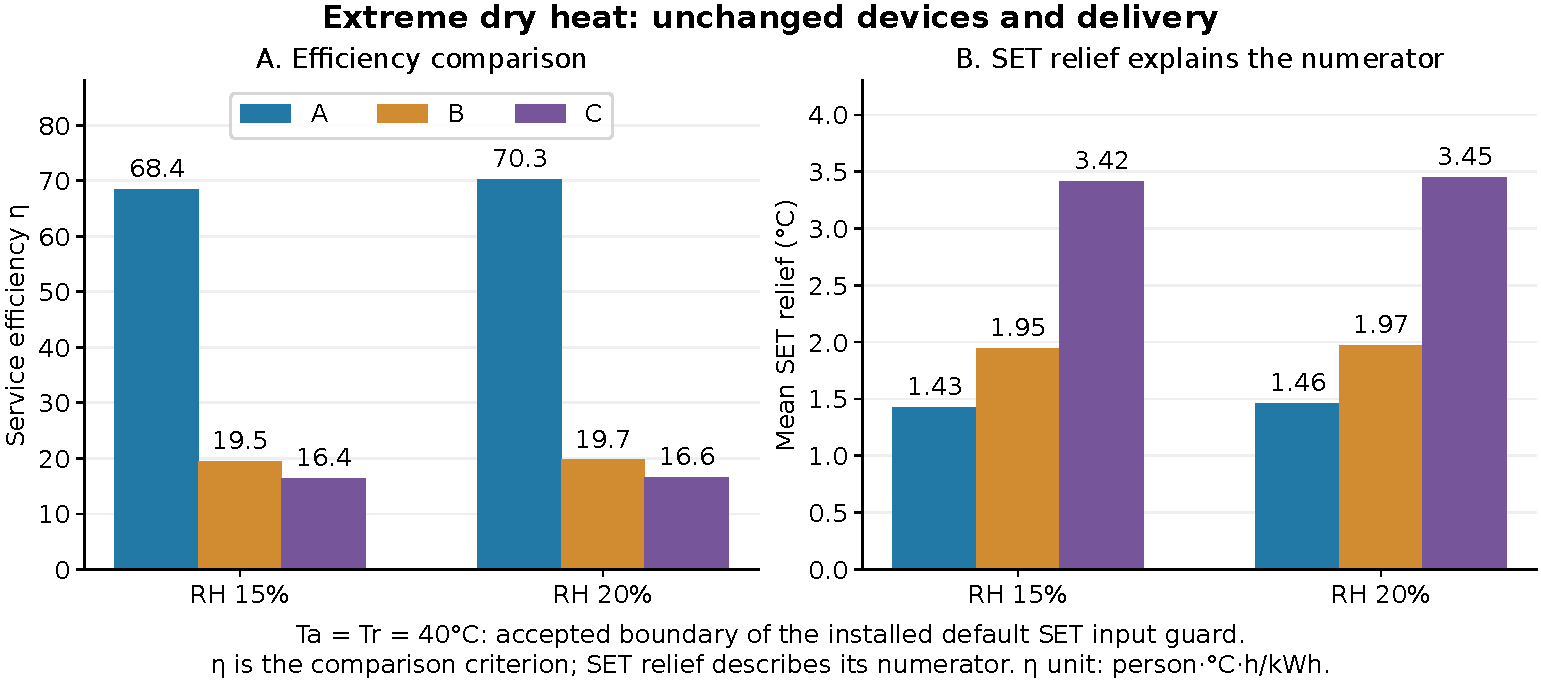
\includegraphics[width=.85\textwidth]{figures/26_extreme_heat.pdf}
\caption{Extreme dry-heat boundary test with the original device powers and delivery profiles. The left panel compares cooling efficiency; the right panel explains its SET-relief numerator. Inputs follow Assumption A4.}
\label{fig:extreme-heat}
\end{figure}

